% metropolis theme from https://github.com/matze/mtheme
\documentclass[xcolor={svgnames,x11names,dvipsnames}]{beamer}
\usepackage{amssymb}
\usepackage{amsthm}
\usepackage{stmaryrd}
\usepackage{wasysym}
\usepackage{mathrsfs}
\usepackage{color}
\usepackage{dsfont}
\usepackage[all]{xy}
\SelectTips{cm}{10}  % Better arrowheads; shamelessly stolen from Anton Geraschenko's notes
\usepackage{float}
\usepackage{mathtools}
\usepackage{array}
\usepackage{scalefnt}
\usepackage{microtype}
\usepackage{ulem}
\usepackage{soul}
\usepackage{hyperref}
\hypersetup{colorlinks=true,urlcolor=RoyalBlue}
\makeatletter
\let\HL\hl
\renewcommand\hl{%
  \let\set@color\beamerorig@set@color
  \let\reset@color\beamerorig@reset@color
  \HL}
\makeatother
\usepackage{colonequals}
\usepackage{xparse}

\usetheme{metropolis}
\definecolor{headerColor}{HTML}{3675a4}
%\definecolor{headerColor}{HTML}{982a78}
\definecolor{secondColor}{HTML}{e42884}
\definecolor{progressBarColor}{HTML}{b19257}
\definecolor{darkAlertColor}{HTML}{b19257}


\usepackage{tikz}
\usetikzlibrary{arrows, decorations.markings}
\tikzstyle{vecArrow} = [thick, decoration={markings,mark=at position
   1 with {\arrow[semithick]{open triangle 45}}},
   double distance=1.4pt, shorten >= 5.5pt,
   preaction = {decorate},
   postaction = {draw,line width=1.4pt, white,shorten >= 4.5pt}]
\tikzstyle{innerWhite} = [semithick, white,line width=1.4pt, shorten >= 4.5pt]
\usetikzlibrary{cd}
% http://tex.stackexchange.com/questions/34921/how-to-overlap-images-in-a-beamer-slide
% http://tex.stackexchange.com/questions/34921/how-to-overlap-images-in-a-beamer-slide
\def\Put(#1,#2)#3{\leavevmode\makebox(0,0){\put(#1,#2){#3}}}
\definecolor{magenta}{HTML}{ff00ff}
%% Actual formatting
\parskip=0.2in \parindent=0in
\allowdisplaybreaks % Allow align environments to split over page breaks
\raggedbottom % Don't leave awkward spaces in the middle of pages


% From Atanas Atanasov: \replacecommand is similar to \providecommand but it initializes the command as necessary even if a previous definition exists.
\newcommand*{\replacecommand}[1]{%
  \providecommand{#1}{}%
  \renewcommand{#1}%
}

\renewcommand{\arraystretch}{1.5}


%% Miscellaneous \newcommand's
\renewcommand{\l}{\overset}
\newcommand{\into}{\hookrightarrow}
\newcommand{\onto}{\twoheadrightarrow}
\newcommand{\tto}{\longrightarrow}
\newcommand{\too}[1]{\overset{#1}\to}
\newcommand{\ttoo}[1]{\overset{#1}\longrightarrow}
\newcommand{\intoo}[1]{\overset{#1}\into}
\newcommand{\ontoo}[1]{\overset{#1}\onto}
\newcommand{\mapstoo}[1]{\overset{#1}\mapsto}
\newcommand{\bto}{\leftarrow}
\newcommand{\btto}{\longleftarrow}
\newcommand{\btoo}[1]{\overset{#1}\bto}
\newcommand{\bttoo}[1]{\overset{#1}\longleftarrow}
\newcommand{\binto}{\hookleftarrow}
\newcommand{\bonto}{\twoheadleftarrow}
\newcommand{\bintoo}[1]{\overset{#1}\binto}
\newcommand{\bontoo}[1]{\overset{#1}\bonto}
% stupid hack to get the open immersion symbol; see http://tex.stackexchange.com/questions/66723/nudging-overset-characters-downwards
\newcommand{\ointo}{\hspace{3pt}\text{\raisebox{-1.5pt}{$\overset{\circ}{\vphantom{}\smash{\text{\raisebox{1.5pt}{$\into$}}}}$}}\hspace{3pt}}
\newcommand{\lu}{\underset}
\newcommand{\bimplies}{\impliedby}
\newcommand{\ints}{\cap}
\newcommand{\intss}{\bigcap}
\newcommand{\union}{\cup}
\newcommand{\unions}{\bigcup}
\newcommand{\djunion}{\sqcup}
\newcommand{\djunions}{\bigsqcup}
\newcommand{\propersubset}{\subsetneq}
\newcommand{\propersupset}{\supsetneq}
\newcommand{\contains}{\supseteq}
\newcommand{\semidirect}{\rtimes}
\newcommand{\isom}{\cong}
\newcommand{\normal}{\triangleleft}
\replacecommand{\dsum}{\oplus}
\newcommand{\dsums}{\bigoplus}
\newcommand{\tensor}{\otimes}
\newcommand{\tensors}{\bigotimes}
\newcommand{\cotensor}{{\,\scriptstyle\square}}
\let\originalbar\bar
\renewcommand{\bar}[1]{{\overline{#1}}}
\newcommand{\rlim}{\mathop{\varinjlim}\limits}
\newcommand{\llim}{\mathop{\varprojlim}\limits}
\newcommand{\x}{\times}
\replacecommand{\st}{\hspace{2pt} : \hspace{2pt}} % used to be \providecommand
\newcommand{\vv}{\vspace{10pt}}
\newcommand{\til}{\widetilde}
\renewcommand{\hat}{\widehat}
\newcommand{\hhat}{\wedge}
\newcommand{\iy}{\infty}
\newcommand{\hteq}{\simeq}
\newcommand{\dd}[2]{\frac{\partial #1}{\partial #2}}
\newcommand{\sm}{\wedge} % stop getting confused about the word "wedge"
\newcommand{\noqed}{\renewcommand{\qedsymbol}{}}
\newcommand{\adjoint}{\dashv}
\newcommand{\wreath}{\wr}
\newcommand{\heart}{\heartsuit}

%http://tex.stackexchange.com/questions/23432/how-to-create-my-own-math-operator-with-limits
\newcommand{\bigast}{\mathop{\vphantom{\sum}\mathchoice%
  {\vcenter{\hbox{\huge *}}}
  {\vcenter{\hbox{\Large *}}}{*}{*}}\displaylimits}


%% \operatorname
\renewcommand{\dim}{\operatorname{dim}}
\newcommand{\diam}{\operatorname{diam}}
\newcommand{\coker}{\operatorname{coker}}
\newcommand{\im}{\operatorname{im}}
\newcommand{\disc}{\operatorname{disc}}
\newcommand{\Pic}{\operatorname{Pic}}
\newcommand{\Der}{\operatorname{Der}}
\newcommand{\ord}{\operatorname{ord}}
\newcommand{\nil}{\operatorname{nil}}
\newcommand{\rad}{\operatorname{rad}}
\newcommand{\ssum}{\operatorname{sum}}
\newcommand{\codim}{\operatorname{codim}}
\newcommand{\cchar}{\operatorname{char}}
\newcommand{\sspan}{\operatorname{span}}
\newcommand{\rank}{\operatorname{rank}}
\newcommand{\Aut}{\operatorname{Aut}}
\newcommand{\Out}{\operatorname{Out}}
\newcommand{\Div}{\operatorname{Div}}
\newcommand{\Gal}{\operatorname{Gal}}
\newcommand{\Hom}{\operatorname{Hom}}
\newcommand{\Mor}{\operatorname{Mor}}
\newcommand{\Vect}{\operatorname{Vect}}
\newcommand{\Fun}{\operatorname{Fun}}
\newcommand{\Iso}{\operatorname{Iso}}
\newcommand{\Map}{\operatorname{Map}}
\newcommand{\Ho}{\operatorname{Ho}}
\newcommand{\Mod}{\operatorname{Mod}}
\newcommand{\Tot}{\operatorname{Tot}}
\newcommand{\cofib}{\operatorname{cofib}}
\newcommand{\fib}{\operatorname{fib}}
\newcommand{\hocofib}{\operatorname{hocofib}}
\newcommand{\hofib}{\operatorname{hofib}}
\newcommand{\Maps}{\operatorname{Maps}}
\newcommand{\Sym}{\operatorname{Sym}}
\newcommand{\Diff}{\operatorname{Diff}}
\newcommand{\Tr}{\operatorname{Tr}}
\newcommand{\Frac}{\operatorname{Frac}}
\renewcommand{\Re}{\operatorname{Re}} % don't like the curly default ones
\renewcommand{\Im}{\operatorname{Im}}
\newcommand{\gr}{{\operatorname{gr}}}
\newcommand{\tr}{\operatorname{tr}}
%\newcommand{\colim}{\operatorname{colim}}
\newcommand{\End}{\operatorname{End}}
\newcommand{\Mat}{\operatorname{Mat}}
\newcommand{\Proj}{\operatorname{Proj}}
\newcommand{\Th}{\operatorname{Thom}}
\newcommand{\Thom}{\operatorname{Thom}}
\newcommand{\Spec}{\operatorname{Spec}}
\newcommand{\Ext}{\operatorname{Ext}}
\newcommand{\Cotor}{\operatorname{Cotor}}
\newcommand{\Tor}{\operatorname{Tor}}
\newcommand{\vol}{\operatorname{vol}}
\newcommand{\Id}{\operatorname{Id}}

%% new operatornames since preamble8
\newcommand{\Set}{\operatorname{Set}}
\newcommand{\Top}{\operatorname{Top}}
\newcommand{\Fin}{\operatorname{Fin}}
\newcommand{\Spaces}{\operatorname{Spaces}}
\newcommand{\Sp}{\operatorname{Sp}}
\newcommand{\Spectra}{\operatorname{Spectra}}
\newcommand{\Spt}{\operatorname{Spt}}
\newcommand{\Comod}{\operatorname{Comod}}
\newcommand{\Spf}{\operatorname{Spf}}
\newcommand{\tmf}{\mathit{tmf}}
\newcommand{\Tmf}{\mathit{Tmf}}
\newcommand{\TMF}{\mathit{TMF}}
\newcommand{\Null}{\operatorname{Null}}
\newcommand{\Fil}{\operatorname{Fil}}
\newcommand{\Sq}{\operatorname{Sq}}
\newcommand{\Stable}{\operatorname{Stable}}
\newcommand{\Poly}{\operatorname{Poly}}
\newcommand{\Cat}{\operatorname{Cat}}
\newcommand{\Orb}{\operatorname{Orb}}
\newcommand{\Exc}{\operatorname{Exc}}
\newcommand{\Part}{\operatorname{Part}}
\newcommand{\Comm}{\operatorname{Comm}}
\newcommand{\Res}{\operatorname{Res}}
\newcommand{\Thick}{\operatorname{Thick}}
\newcommand{\red}{{\operatorname{red}}}
\providecommand{\SH}{\mathrm{SH}}
\providecommand{\fil}{{\mathrm{fil}}}

\newcommand{\mmf}{\mathit{mmf}}
\newcommand{\Sm}{\operatorname{Sm}}
\newcommand{\Var}{\operatorname{Var}}
\newcommand{\Frob}{\operatorname{Frob}}
\newcommand{\Rep}{\operatorname{Rep}}
\newcommand{\Ch}{\operatorname{Ch}}
\newcommand{\Shv}{\operatorname{Shv}}
\newcommand{\Corr}{\operatorname{Corr}}
\newcommand{\Span}{\operatorname{Span}}
\newcommand{\Sch}{\operatorname{Sch}}
\newcommand{\ev}{\operatorname{ev}}
\newcommand{\Homog}{\operatorname{Homog}}
\newcommand{\conn}{\operatorname{conn}}
\newcommand{\type}{\operatorname{type}}
\newcommand{\num}{\operatorname{num}}
\newcommand{\Aff}{\operatorname{Aff}}
\newcommand{\Psh}{\operatorname{Psh}}
\newcommand{\sk}{\operatorname{sk}}
\newcommand{\cosk}{\operatorname{cosk}}
\newcommand{\Cart}{\operatorname{Cart}}

\newcommand{\Br}{\operatorname{Br}}
\newcommand{\BW}{\operatorname{BW}}
\newcommand{\Cl}{\operatorname{Cl}}
\newcommand{\Conf}{\operatorname{Conf}}
\newcommand{\Alg}{\operatorname{Alg}}
\newcommand{\CAlg}{\operatorname{CAlg}}
\newcommand{\Lie}{\operatorname{Lie}}
\newcommand{\Coalg}{\operatorname{Coalg}}
\newcommand{\Ab}{\operatorname{Ab}}
\newcommand{\Ind}{\operatorname{Ind}}
\newcommand{\ind}{\operatorname{ind}}
\newcommand{\Fix}{\operatorname{Fix}}
\newcommand{\ho}{\operatorname{ho}}
\newcommand{\coeq}{\operatorname{coeq}}
\newcommand{\CMon}{\operatorname{CMon}}
\newcommand{\Sing}{\operatorname{Sing}}
\newcommand{\Inj}{\operatorname{Inj}}
\newcommand{\StMod}{\operatorname{StMod}}
\newcommand{\Loc}{\operatorname{Loc}}
\newcommand{\Free}{\operatorname{Free}}
\newcommand{\Art}{\operatorname{Art}}
\newcommand{\Gpd}{\operatorname{Gpd}}
\newcommand{\Def}{\operatorname{Def}}
\newcommand{\Hyp}{\operatorname{Hyp}}
\newcommand{\Pre}{\operatorname{Pre}}
\newcommand{\Lat}{\operatorname{Lat}}
\newcommand{\Coords}{\operatorname{Coords}}
\newcommand{\cone}{\operatorname{cone}}
\newcommand{\Spc}{\operatorname{Spc}}
\newcommand{\QCoh}{\operatorname{QCoh}}
\newcommand{\height}{\operatorname{ht}}
\newcommand{\Sub}{\operatorname{Sub}}
\newcommand{\Cone}{\operatorname{Cone}}
\newcommand{\Cocone}{\operatorname{Cocone}}
\newcommand{\Ran}{\operatorname{Ran}}
\newcommand{\Lan}{\operatorname{Lan}}
\newcommand{\LieAlg}{\operatorname{LieAlg}}
\newcommand{\Com}{\operatorname{Com}}
\newcommand{\CoAlg}{\operatorname{CoAlg}}
\newcommand{\Prim}{\operatorname{Prim}}
\newcommand{\Coh}{\operatorname{Coh}}
\newcommand{\FormalGrp}{\operatorname{FormalGrp}}
\newcommand{\Fact}{\operatorname{Fact}}
\renewcommand{\Bar}{\operatorname{Bar}}
\newcommand{\Cobar}{\operatorname{Cobar}}
\newcommand{\Ad}{\operatorname{Ad}}
\newcommand{\Moduli}{\operatorname{Moduli}}
\newcommand{\dgla}{\operatorname{dgla}}
\newcommand{\obl}{\operatorname{obl}}
\newcommand{\ob}{\operatorname{ob}}
\newcommand{\IndCoh}{\operatorname{IndCoh}}
\newcommand{\Cocomm}{\operatorname{Cocomm}}
\newcommand{\PreStk}{\operatorname{PreStk}}
\newcommand{\FormGrp}{\operatorname{FormGrp}}
\newcommand{\FormMod}{\operatorname{FormMod}}
\newcommand{\Grp}{\operatorname{Grp}}
\newcommand{\CommAlg}{\operatorname{CommAlg}}
\newcommand{\CoComm}{\operatorname{CoComm}}
\newcommand{\IndSch}{\operatorname{IndSch}}
\newcommand{\Dist}{\operatorname{Dist}}
\newcommand{\Triv}{\operatorname{Triv}}
\newcommand{\Oper}{\operatorname{Oper}}
\newcommand{\Bij}{\operatorname{Bij}}
\newcommand{\Syl}{\operatorname{Syl}}
\newcommand{\Inn}{\operatorname{Inn}}
\newcommand{\Emb}{\operatorname{Emb}}
\newcommand{\Gr}{\operatorname{Gr}}
\newcommand{\CRing}{\operatorname{CRing}}
\newcommand{\sSet}{\operatorname{sSet}}
\newcommand{\et}{\text{\'et}}
\newcommand{\Sh}{\operatorname{Sh}}
\newcommand{\Nil}{\operatorname{Nil}}
\newcommand{\Cech}{\v Cech}
\newcommand{\Stacks}{\operatorname{Stacks}}
\newcommand{\Pin}{\operatorname{Pin}}
\newcommand{\sgn}{\operatorname{sgn}}
%END



%% \A etc.
\newcommand{\A}{\mathbb{A}}
\replacecommand{\C}{\mathbb{C}}
\newcommand{\CP}{\mathbb{C}\mathrm{P}}
\newcommand{\E}{\mathbb{E}}
\newcommand{\F}{\mathbb{F}}
\replacecommand{\G}{\mathbb{G}}
\renewcommand{\H}{\mathbb{H}}
\newcommand{\K}{\mathbb{K}}
\newcommand{\M}{\mathbb{M}}
\newcommand{\N}{\mathbb{N}}
\renewcommand{\P}{\mathbb{P}}
\newcommand{\Q}{\mathbb{Q}}
\newcommand{\R}{\mathbb{R}}
\newcommand{\RP}{\mathbb{R}\mathrm{P}}
\newcommand{\V}{\vee}
\newcommand{\T}{\mathbb{T}}
\providecommand{\U}{\mathscr{U}}
\newcommand{\Z}{\mathbb{Z}}
\newcommand{\e}{\mathfrak{g}}
\newcommand{\m}{\mathfrak{m}}
\newcommand{\n}{\mathfrak{n}}
\newcommand{\p}{\mathfrak{p}}
\newcommand{\q}{\mathfrak{q}}
\renewcommand{\t}{\mathfrak{t}}



%% Large parentheses, etc.
\newcommand{\pa}[1]{\left( {#1} \right)}
\newcommand{\br}[1]{\left[ {#1} \right]}
\newcommand{\cu}[1]{\left\{ {#1} \right\}}
\newcommand{\ab}[1]{\left| {#1} \right|}
\newcommand{\an}[1]{\left\langle {#1}\right\rangle}
\newcommand{\fl}[1]{\left\lfloor {#1}\right\rfloor}
\newcommand{\ceil}[1]{\left\lceil {#1}\right\rceil}
\newcommand{\tf}[1]{{\textstyle{#1}}}
\newcommand{\patf}[1]{\pa{\textstyle{#1}}}



%% Weird constructions
\renewcommand{\mp}{\ \raisebox{5pt}{\text{\rotatebox{180}{$\pm$}}}\ }
\renewcommand{\d}[1]{\ss \mathrm{d}#1}
\newcommand{\imod}{\hspace{-7pt}\pmod}
%\renewcommand{\check}[1]{\overset{\smile}{#1}}



%% Better versions of existing commands
\renewcommand{\epsilon}{\varepsilon}
\let\originalphi=\phi
\renewcommand{\phi}{{\mathchoice{\raisebox{2pt}{\ensuremath\varphi}}{\raisebox{2pt}{\!\! \ensuremath\varphi}}{\raisebox{1pt}{\scriptsize$\varphi$}}{\varphi}}}
\newcommand{\ph}{{\color{white}.\!}}
\newcommand{\tspacer}{{\ensuremath{\color{white}\Big|\!}}}
\newcommand{\chii}{\raisebox{2pt}{\ensuremath\chi}}

% from http://mbork.pl/2009-04-27_Fun_with_quantifiers_%28en%29
\let\originalchi=\chi
\renewcommand{\chi}{{\!{\mathchoice{\raisebox{2pt}{
$\originalchi$}}{\!\raisebox{2pt}{
$\originalchi$}}{\raisebox{1pt}{\scriptsize$\originalchi$}}{\originalchi}}}}

\let\originalforall=\forall
\renewcommand{\forall}{\ \originalforall}

\let\originalexists=\exists
\renewcommand{\exists}{\ \originalexists}

\let\realcheck\check
\newcommand{\vH}{\realcheck{H}}



% quote block: \begin{qu}{leftmargin}{rightmargin}{  ...  }
\newenvironment{qu}[2]
{\begin{list}{}
	  {\setlength\leftmargin{#1}
	  \setlength\rightmargin{#2}}
	  \item[]\footnotesize}
		  {\end{list}}


\newenvironment{titleblock}
{\begin{mdframed}[linecolor=black!20,backgroundcolor=black!15]\begin{center}}
{\end{center}\end{mdframed}}

\newenvironment{shadedblock}[1][5in]
{\bigskip\begin{mdframed}[align=center,userdefinedwidth=#1,linecolor=white,backgroundcolor=black!5]}{\end{mdframed}}

\newenvironment{shadedtitleblock}[2][5in]
{\begin{mdframed}[align=center,userdefinedwidth=#1,linecolor=white,backgroundcolor=black!15]\sc #2\end{mdframed}\begin{mdframed}[align=center,userdefinedwidth=#1,linecolor=white,backgroundcolor=black!5]}{\end{mdframed}}

\newcommand{\shadedheader}[1]{\vspace{25pt}\begin{mdframed}[linecolor=black!20,backgroundcolor=black!5]\sc #1\end{mdframed}\vspace{10pt}}





%%%%%%%%%%%%%%%%%%%%%%%%%
%% newcommands that require certain packages

\newcommand{\itext}{\shortintertext} % requires mathtools
\makeatletter
\@ifundefined{resetu}{ % revert to \u as text accent by defining \resetu
	\renewcommand{\u}{\underbracket[0.7pt]} % requires mathtools
}
\makeatother
\makeatletter
\@ifundefined{resetO}{ % revert to \O as text accent by defining \resetO
	\renewcommand{\O}{\mathcal{O}}
}
\makeatother
\makeatletter
\@ifundefined{resetk}{ % revert to \O as text accent by defining \resetO
	\renewcommand{\k}{\Bbbk}
}
\makeatother



%%%%%%%%%%%%%%%%%%%%

% Colors
% Now this preamble doesn't cause errors when there is no \usepackage{color}
% (you just can't use these commands)
\makeatletter
%\@ifundefined{mathds}{
%	\newcommand{\Id}{Id}
%	}{
%	\newcommand{\Id}{\mathds{1}} % requires mathds
%	}
\@ifundefined{sethlcolor}{
	\newcommand{\fixmehl}[2]{\underline{#1}\marginpar{\raggedright\smaller\smaller #2}}
	}{\@ifundefined{marginnote}{
		\newcommand{\highlight}[1]{\ifmmode{\text{\sethlcolor{llgray}\hl{$#1$}}}\else{\sethlcolor{llred}\hl{#1}}\fi}
		\newcommand{\fixmehl}[2]{\highlight{#1}\marginpar{\raggedright\smaller\smaller\color{maroon} #2}}
		}{
		\newcommand{\highlight}[1]{\ifmmode{\text{\sethlcolor{llgray}\hl{$#1$}}}\else{\sethlcolor{llred}\hl{#1}}\fi}
		\newcommand{\fixmehl}[2]{\marginnote{\smaller \smaller\color{maroon} #2}{\highlight{#1}}}
		}
	}
\@ifundefined{xy}{}{
	\SelectTips{cm}{10}  % Better arrowheads
}
\@ifundefined{color}{}{
	\definecolor{darkgreen}{RGB}{0,70,0}
	\definecolor{dgreen}{RGB}{0,100,0}
	\definecolor{purple}{RGB}{120,00,120}
	\definecolor{gray}{RGB}{100,100,100}
	\definecolor{mgreen}{RGB}{0,150,0}
	\definecolor{dgreen}{RGB}{0,100,0}
	\definecolor{llgray}{RGB}{230,230,230}
	\definecolor{llred}{RGB}{237,228,228}
	\definecolor{lgreen}{RGB}{100,200,100}
	\definecolor{mgray}{RGB}{150,150,150}
	\definecolor{lgray}{RGB}{190,190,190}
	\definecolor{maroon}{RGB}{150,0,0}
	\definecolor{lblue}{RGB}{120,170,200}
	\definecolor{mblue}{RGB}{65,105,225}
	\definecolor{dblue}{RGB}{0,56,111}
	\definecolor{orange}{RGB}{255,165,0}
	\definecolor{brown}{RGB}{177,84,15}
	\definecolor{rose}{RGB}{135,0,52}
	\definecolor{gold}{RGB}{177,146,87}
	\definecolor{dred}{RGB}{135,19,19}
	\definecolor{mred}{RGB}{194,28,28}
	\newcommand{\edit}[1]{{\it{\color{gray}#1}}}
	\newcommand{\fixme}[1]{{\color{maroon}\it{#1}}}
	\newcommand{\citeme}[2][\!\!]{{\color{orange}[#2~\textit{#1}]}}
	\newcommand{\later}[1]{{\color{dgreen}#1}}
	\newcommand{\corr}[1]{{\color{red}\itshape #1}}
	\newcommand{\question}[1]{\itshape{\color{blue}#1}\upshape}
}
\@ifundefined{substack}{}{
    \newcommand{\attop}[1]{{\let\textstyle\scriptstyle\let\scriptstyle\scriptscriptstyle\substack{#1}}}
    \renewcommand{\atop}[1]{{\let\scriptstyle\textstyle\let\scriptscriptstyle\scriptstyle\substack{#1}}}
}


\@ifundefined{devanagari}{\newcommand{\ta}{{\tt ta}}}{\newcommand{\ta}{\text{{\dn t}}}}

\makeatother

%%%%%%%%%%%%%%%%%%%%

\newcommand{\tabentry}[1]{\renewcommand{\arraystretch}{1}\begin{tabular}{c}#1\end{tabular}}


\newcommand{\margin}[1]{\marginpar{\raggedright \scalefont{0.7}#1}} % requires scalefnt

% require package pigpen and xy
\newcommand{\pullback}{\ar@{}[rd]|<<{\text{\pigpenfont A}}}
\newcommand{\pushout}{\ar@{}[rd]|>>{\text{\pigpenfont I}}}

% requires xy
% Somehow these don't work when placed earlier in the preamble. Maybe something
% about the \makeatletter thing
\newcommand{\longleftrightarrows}{\xymatrix@1@C=16pt{
\ar@<0.4ex>[r] & \ar@<0.4ex>[l]
}}
\newcommand{\longrightrightarrows}{\xymatrix@1@C=16pt{
\ar@<0.4ex>[r]\ar@<-0.4ex>[r] & 
}}
\newcommand{\mapstto}{\,\xymatrix@1@C=16pt{
\ar@{|->}[r] & 
}\,}
\newcommand{\mapsttoo}[1]{\xymatrix@1@C=16pt{
\ar@{|->}[r]^-{#1} & 
}}
\newcommand{\rightrightrightarrows}{\xymatrix@1@C=16pt{
\ar[r]\ar@<0.8ex>[r]\ar@<-0.8ex>[r] & 
}}
\newcommand{\longleftleftarrows}{\xymatrix@C=16pt{
 & \ar@<0.4ex>[l]\ar@<-0.4ex>[l]
}}
\newcommand{\leftleftleftarrows}{\xymatrix@1@C=16pt{
 & \ar[l]\ar@<0.8ex>[l]\ar@<-0.8ex>[l]
}}
\newcommand{\leftleftleftleftarrows}{\xymatrix@1@C=16pt{
 & \ar@<0.8ex>[l]\ar@<0.3ex>[l]\ar@<-0.3ex>[l]\ar@<-0.8ex>[l]
}}
\newcommand{\lcircle}{\ar@(ul,dl)} % arrow circle to the left of the node
\newcommand{\rcircle}{\ar@(ur,dr)}
\newcommand{\intto}{\ \xymatrix@1@C=16pt{
\ar@{^(->}[r] & 
}}

\newcommand{\eva}[1]
   {{\color{Periwinkle}\it #1}}
\newcommand{\EvaNote}[1]
   {\marginpar{\raggedright\smaller \smaller \color{Periwinkle}#1}}


\makeatletter
\newcommand{\switchmargin}{
\if@reversemargin
\normalmarginpar
\else
\reversemarginpar
\fi
}
\makeatother
\newcommand{\highlighteva}[1]{\ifmmode{\text{\sethlcolor{Lavender}\hl{$#1$}}}\else{\sethlcolor{Lavender}\hl{#1}}\fi}
\newcommand{\EvaNoteHl}[2]{\marginnote{\smaller \smaller \color{Periwinkle}
#2}{\highlighteva{#1}}\switchmargin}

\newcommand\spoke{{\scaleobj{1.2}{\Yright}}}

%  vim:ft=tex

\setbeamersize{text margin right=20pt}
\setbeamertemplate{footline}[frame number]
\expandafter\def\expandafter\insertshorttitle\expandafter{%
  \insertshorttitle\hfill%
  \insertframenumber\,/\,\inserttotalframenumber}

\newcommand{\fiber}{\operatorname{fiber}}
\newcommand{\colim}{\operatorname{colim}}

\setlength{\paperwidth}{5in}
\setlength{\paperheight}{6in}

\definecolor{darkgreen}{HTML}{008400}
\newcommand{\cmd}{}
\RenewDocumentCommand{\cmd}{v}{{\color{darkgreen}\texttt{#1}}}
\newcommand{\easycmd}[1]{{\tt \color{darkgreen}#1}}

\title{{\tt git} and other fun}
\date{June 18, 2026}
\author{Eva Belmont}
\begin{document}
\normalem

\renewcommand{\tabentry}[1]{\renewcommand{\arraystretch}{1.0}\hspace{-5pt}\begin{tabular}{l}#1\end{tabular}}

\newcommand{\argforrandom}{}
\theoremstyle{newtextthm}
\newtheorem{helperforrandom}[theorem]{\argforrandom}
\newtheorem*{helperforrandomstar}{\argforrandom}
\newenvironment{random}[1]{\renewcommand{\argforrandom}{#1}\begin{helperforrandom}}{\end{helperforrandom}}
\newenvironment{randomstar}[1]{\renewcommand{\argforrandom}{#1}\begin{helperforrandomstar}}{\end{helperforrandomstar}}

\renewcommand{\red}[1]{{\color{secondColor}#1}}

\setbeamercolor{normal text}{fg=headerColor!90, bg=black!0}
\setbeamercolor{alerted text}{fg=progressBarColor}
\setbeamercolor{block title example}{fg=headerColor!90}
\setbeamercolor{section title}{fg=headerColor}
\setbeamercolor{title separator}{bg=progressBarColor}
\setbeamercolor{progress bar}{fg=progressBarColor}
\setbeamercolor{title separator}{fg=progressBarColor}
\setbeamercolor{block body}{bg=black!5}
\setbeamercolor{block title}{bg=black!10}
\setbeamercolor{title}{fg=headerColor}
\setbeamercolor{author}{fg=black}
\setbeamercolor{date}{fg=black}
\setbeamercolor{institute}{fg=black}
\maketitle
%\setbeamertemplate{footline}{}
\metroset{numbering=fraction}  % for the X/Y in the lower right
%\metroset{numbering=none}
\sethlcolor{Yellow}

%%%% BEGIN

\begin{frame} {A new beginning!}
\end{frame}

\begin{frame} {Exercise 1}
\textbf{Step 1.} Open a terminal
\begin{columns}[t]
\begin{column}{0.5\textwidth}
\begin{block}{Windows}
Windows Key + r

Type {\tt cmd} and hit enter
\end{block}
\vspace{10pt}
\begin{block}{Windows + WSL}
Open the Ubuntu app
\\{\color{mgray}and later follow the Linux instructions if given}
\end{block}

% also accepts forward slashes except where it doesn't
\end{column}
\begin{column}{0.5\textwidth}
\begin{block}{MacOS}
Cmd + space

Type {\tt terminal} and hit enter
\end{block}
\end{column}
\end{columns}

\vspace{20pt}

\textbf{Step 2.} Keyboard mash and hit enter

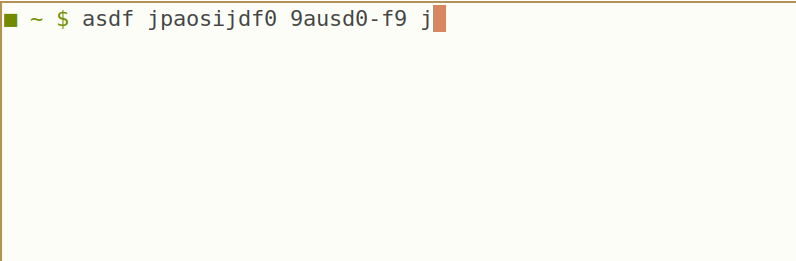
\includegraphics[width=200pt]{images/asdf1.png}
\end{frame}

\begin{frame}[fragile] {What happened? (take 1)}
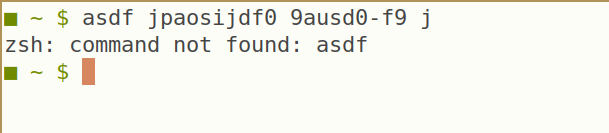
\includegraphics[width=150pt]{images/asdf.png}
\vspace{40pt}
\begin{itemize} 
\item The shell tried to run the program \cmd{asdf} with arguments \cmd{jpaosijdf0}, \cmd{9ausd0-f9}, and \cmd{j}.
\pause
\item But there is no program called \cmd{asdf} \  :(
\end{itemize}
\end{frame}

\begin{frame} [fragile] {Commands and arguments: common patterns}
\begin{columns}[t]
\begin{column}{0.5\textwidth}
\begin{block}{Windows \tt{cmd}}
\cmd{dir}
\vspace{15pt}

\cmd{dir Documents}
\vspace{15pt}

\cmd{dir /w Documents}
\end{block}
% also accepts forward slashes except where it doesn't
\end{column}
\begin{column}{0.5\textwidth}
\begin{block}{{\tt zsh}, {\tt bash} (MacOS/ Linux)}
\cmd{ls}
\vspace{15pt}

\cmd{ls Documents}
\vspace{15pt}

\cmd{ls -l Documents}
\vspace{15pt}

\cmd{ls --help}
\end{block}
\end{column}
\end{columns}
\end{frame}

\begin{frame}[fragile] {Commands and arguments: more complicated syntax examples}
\color{darkgreen}
\begin{verbatim}
cargo run --release --features concurrent


sage -python -m pip install pycryptosat


g++ -g exponents.cpp Fp.cpp mon_index.cpp steenrod.cpp \
    steenrod_init.cpp stmain.cpp -std=c++11 \
    -I./ -Wall -Wfatal-errors -O2 -fopenmp -omr_st

\end{verbatim}
\end{frame}

\begin{frame}[fragile] {Exercise 2}
\begin{columns}[t]
\begin{column}{0.5\textwidth}
\begin{block}{Windows}
\begin{enumerate} 
\item Use a text editor (e.g. notepad) to write the following basic script in a file called
{\tt asdf.bat}:

\vspace{10pt}
{\tt echo hello}
\item Try to run your script
\end{enumerate}
\end{block}
\end{column}
\begin{column}{0.5\textwidth}
\begin{block}{MacOS/ Linux}
\begin{enumerate} 
\item Use a text editor to save this basic script as a file called {\tt asdf}
(no extension)
\begin{verbatim}
#!/bin/bash
echo hello
\end{verbatim}
\item (``set executable permission'')
\cmd{chmod +x asdf}
\item Try to run your script
\end{enumerate}
\end{block}

%\pause

%But it works if you specify the full path, e.g.
%\\{\tt \$ /home/ebelmont/asdf}
\end{column}
\end{columns}
\end{frame}


\begin{frame}[fragile] {What happened? (take 2)}
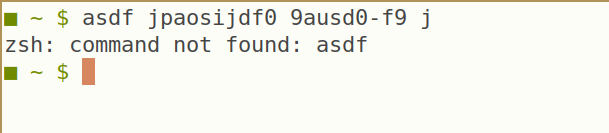
\includegraphics[width=150pt]{images/asdf.png}
\vspace{40pt}
\begin{itemize} 
\item The shell tried to run the program \cmd{asdf} with arguments \cmd{jpaosijdf0}, \cmd{9ausd0-f9}, and \cmd{j}.
\item {\color{Maroon}But there is \textbf{still} no program called \cmd{asdf}???}
\end{itemize}
\textbf{Question:} Where does it look for \cmd{asdf}?

\pause
\textbf{(Partial) answer:} 

\begin{columns}[t]
\begin{column}{0.5\textwidth}
\begin{block}{Windows {\tt cmd}}
\cmd{echo %path%}

(but Windows {\tt cmd} actually does look in your current directory first)
\end{block}
\end{column}
% Note: demo mv asdf into path
% which
\begin{column}{0.5\textwidth}

\begin{block}{{\tt zsh}, {\tt bash} (MacOS/ Linux)}
\cmd{echo $PATH}
\vspace{10pt}
\end{block}
\end{column}
\end{columns}
\end{frame}




\begin{frame}[fragile]{Digression on paths}
\textbf{Absolute paths}
\begin{columns}[t]
\begin{column}{0.53\textwidth}
\begin{block}{Windows}
\verb=C:\Users\ebelmont\Documents = 

\verb=A:\ =

\ 
\end{block}
% also accepts forward slashes except where it doesn't
\end{column}
\begin{column}{0.48\textwidth}
\begin{block}{MacOS/ Linux}
\verb=/Users/ebelmont/Documents=

\verb=/=

\verb=~/Documents=
\end{block}
\end{column}
\end{columns}

\textbf{Relative paths}
\begin{columns}[t]
\begin{column}{0.5\textwidth}
\begin{block}{Windows}
\verb=Documents=
\end{block}
\end{column}
\begin{column}{0.5\textwidth}
\begin{block}{MacOS/ Linux}
\verb=Documents=
\end{block}
\end{column}
\end{columns}
Does this mean \verb=/Documents= or \verb=/Users/ebelmont/Documents=?
\\Interpreted relative to the ``current directory''.
\end{frame}

\begin{frame} [fragile] {Every program has a ``current directory''}
%\textbf{Example 1:} A python program can see its own current directory via
%\vspace{-10pt}
%\begin{center}
%{\tt import os}
%\\{\tt \ \ os.getcwd()}
%\end{center}

Change directory in the shell and view current directory
\vspace{-10pt}

\begin{columns}[t]
\begin{column}{0.5\textwidth}
\begin{block}{Windows {\tt cmd}}
\cmd{cd Documents}

\cmd{cd}

\cmd{cd ..}

\cmd{cd}
\end{block}
\end{column}
\begin{column}{0.5\textwidth}

\begin{block}{{\tt zsh}, {\tt bash} (MacOS/ Linux)}
\cmd{cd Documents}

\cmd{pwd}

\cmd{cd ..}

\cmd{pwd}
\end{block}
\end{column}
\end{columns}

\vspace{20pt}


\begin{block}{. and ..}
\verb=./Documents=  (same as just \verb=Documents= in the current directory)

\verb=../Documents= (the Documents folder in the parent directory)
\end{block}
% these are absolute paths!

%\begin{block}{Exercise 2}
%What is the parent directory of {\tt /}?
%\\(Windows version: what is the parent directory of \verb=C:\=)
%\end{block}

\vspace{30pt}

\pause
\begin{block}{Exercise 3}
\begin{enumerate} 
\item Navigate to the directory of a project you've worked on recently.
\item List the files there.
\item Go back to your home directory (e.g. {\tt /Users/yourname}).
\end{enumerate}
\end{block}
\end{frame}

\begin{frame}[fragile] {USE TAB COMPLETION}

\begin{block}{Exercise 4}
Type
\\\cmd{cd Doc}
\\Stop, and hit Tab.
\end{block}
\pause
\begin{block}{Exercise 5}
Do Exercise 3 again but using tab completion. (Bonus: what is the fewest
keystrokes required?)

%{\color{Green}Bored?}
\vspace{20pt}
{\color{mgray}Exercise 3:}
{\color{mgray}
\begin{enumerate} 
\item \color{mgray} Navigate to the directory of a project you've worked on recently.
\item  List the files there.
\item Go back to your home directory (e.g. {\tt /Users/yourname}).
\end{enumerate}
}

\end{block}
\end{frame}


\begin{frame}[fragile] {What happened? (take 3)}
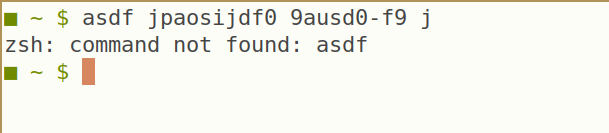
\includegraphics[width=150pt]{images/asdf.png}
\begin{itemize} 
\item The shell tried to run the program \cmd{asdf} with arguments \cmd{jpaosijdf0}, \cmd{9ausd0-f9}, and \cmd{j}.
\item But there is \textbf{still} no program called \cmd{asdf}?
\end{itemize}
\textbf{Question:} Where does it look for \cmd{asdf}?

\pause
\textbf{Answer:}  {\color{Maroon} If it looks like a path (has a /) then it
executes the path.

If not, it looks in your PATH.}
\vspace{20pt}

\begin{block}{Exercise 6}
Without moving your script {\tt asdf} or changing your {\tt PATH}, execute the
script. (Can you do it with tab completion?)
\end{block}
\pause

Best answer (useful pattern):
\\\cmd{./asdf}
\end{frame}

\begin{frame}[fragile] {More on PATH and environment variables}
PATH is a per-process variable (each shell instance has its own PATH) but it can
be set on different levels.
\begin{itemize} 
\item Per command:
\\\cmd{PATH=. asdf}
\\or
\\\cmd{PATH=$PATH:. asdf} \hspace{10pt} {\color{mgray}$\leftarrow$ doesn't wipe
out rest of PATH}
\item Per shell session:
\\\cmd{export PATH=$PATH:.}
\\\cmd{asdf}

\begin{block}{Exercise 7}
What is the difference between \cmd{PATH=$PATH:.} and \cmd{PATH=.:$PATH}?
\end{block}
\item Per user: edit the file {\tt \textasciitilde/.bashrc} (for bash) or {\tt
\textasciitilde/.zshrc} (zsh)
and add the line 
\\{\tt export PATH=\$PATH:.} 
\\This affects all \emph{new} shell sessions made after the change.
\\{\hspace{10pt}\color{mgray}This is just an example\dots putting ``.'' in your
PATH permanently is not a good idea.}
\\Many install scripts do this (replacing ``.'' by wherever the new programs are
installed).
\end{itemize}
\pause

{\tt PATH} is just one of many per-process \emph{environment variables}. Setting
them works the same way.
\end{frame}

\begin{frame} {Troubleshooting lesson \#1: Make sure you're in the right directory}
~\hspace{-20pt}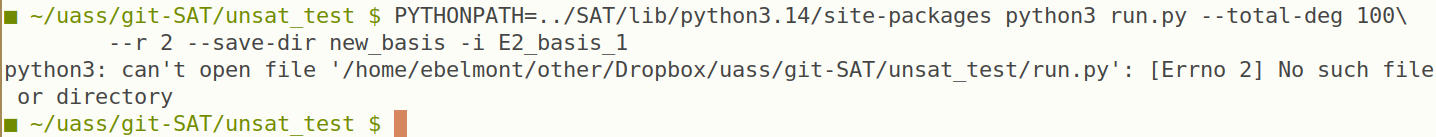
\includegraphics[width=340pt]{images/wrong_dir.png}
\end{frame}

\begin{frame} {Troubleshooting lesson \#2: The documentation might be wrong (or
not apply to you, or take shortcuts)}
Literally a screenshot of the documentation:

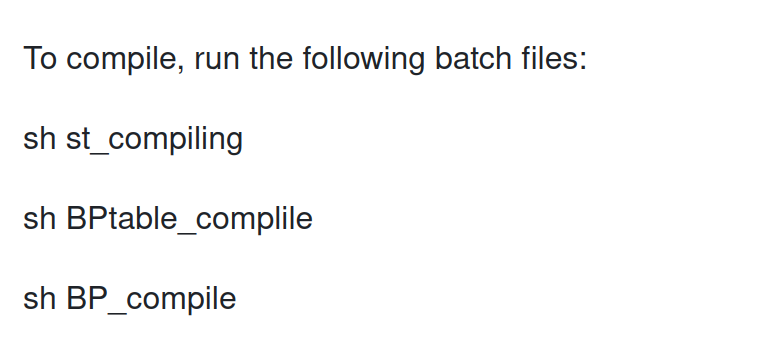
\includegraphics[width=200pt]{images/complile.png}

My attempt:

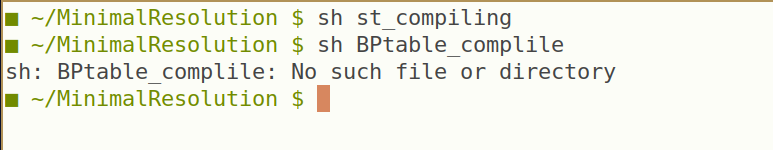
\includegraphics[width=200pt]{images/complile2.png}

\vspace{30pt}

{\color{Purple}Moral of the story: tab completion?}
\end{frame}

\begin{frame}{Troubleshooting lesson \#3: Error messages are clues}
\only<1>{
~\hspace{-15pt}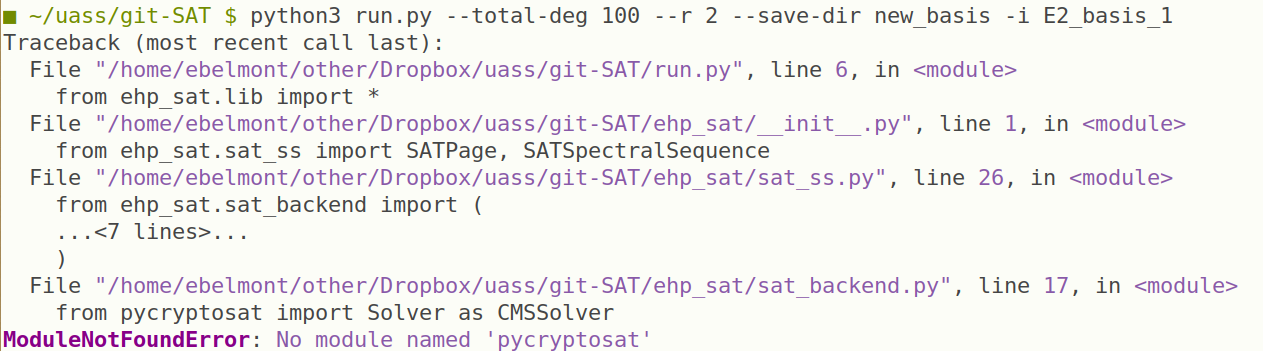
\includegraphics[width=340pt]{images/no_pycryptosat.png}
}
\only<2>{
~\hspace{-15pt}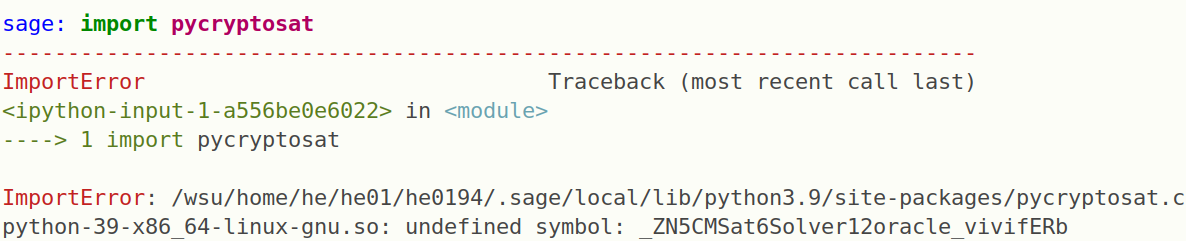
\includegraphics[width=340pt]{images/symbol.png}
}
\end{frame}


\begin{frame} {Upshot}
\begin{itemize} 
\item Commands are just programs
\item ``Command not found:'' 99\% of the time
\begin{itemize} 
\item typo, or
\item {\tt \$PATH} issue.
\end{itemize}
Extremely figure-out-able
\item ``No such file or directory'': often a relative path confusion (you're
probably telling it to look in the wrong place)
\vspace{30pt}
\item {\color{Purple}Also use tab completion!}
\end{itemize}
\end{frame}


\begin{frame}[fragile] {Application: python virtual environments}
Virtual environments are a way to ``install python modules locally to a
project'' {\scalefont{0.8}(instead of making them available every time you run
python)}.

\vspace{-5pt}
%Documentation says:
\vspace{-10pt}
\begin{itemize} 
\item \easycmd{cd path/to/project}
\item \easycmd{python -m venv .} {\hspace{20pt} \color{mgray} (installs the virtual
env---do this once)}
\item Activate the virtual environment:
\\\easycmd{source ./bin/activate} {\hspace{20pt} \color{mgray} (runs the script ./bin/activate)}
\\(needs to be redone every time you have a new terminal where you want to work on the project)
\item Now you can install modules:
\\\easycmd{pip install yourmodule}
\\and they will be available only if {\tt activate} has been run.
\end{itemize}

\pause

\vspace{-5pt}
What happened?
\vspace{-10pt}
\begin{itemize} 
\item \easycmd{which pip} or \easycmd{which python} shows it has modified the {\tt \$PATH} to
use the one in {\tt ./bin/}
\item Packages get installed to {\tt ./lib}, not system-wide
\item Looking at the script {\tt ./bin/activate}, we see 
\begin{verbatim}
export VIRTUAL_ENV=/home/ebelmont/tmp/temp-venv
[...]
PATH="$VIRTUAL_ENV/"bin":$PATH"
export PATH
\end{verbatim}
in addition to some less important stuff.
\end{itemize}
\vspace{-10pt}
{\bf Not magic, just environment variables!}
\end{frame}

\begin{frame} [fragile] {Part 2: Install git}
\begin{itemize} 
\item MacOS: type \cmd{git} in the terminal. It should offer to install git.
\vspace{20pt}
\item Windows without WSL: install from
\\\url{gitforwindows.org}
\vspace{20pt}
\item Windows with WSL: \cmd{git} should already be installed. (Type \cmd{git} in
the WSL prompt; you should get a usage message, not ``command not found.'')
\vspace{100pt}
\item {\color{Purple} Pet peeve: git $\neq$ GitHub}
\end{itemize}
\end{frame}

\begin{frame} {Git: basic model}
\only<1>{\vspace{24pt}\centerline{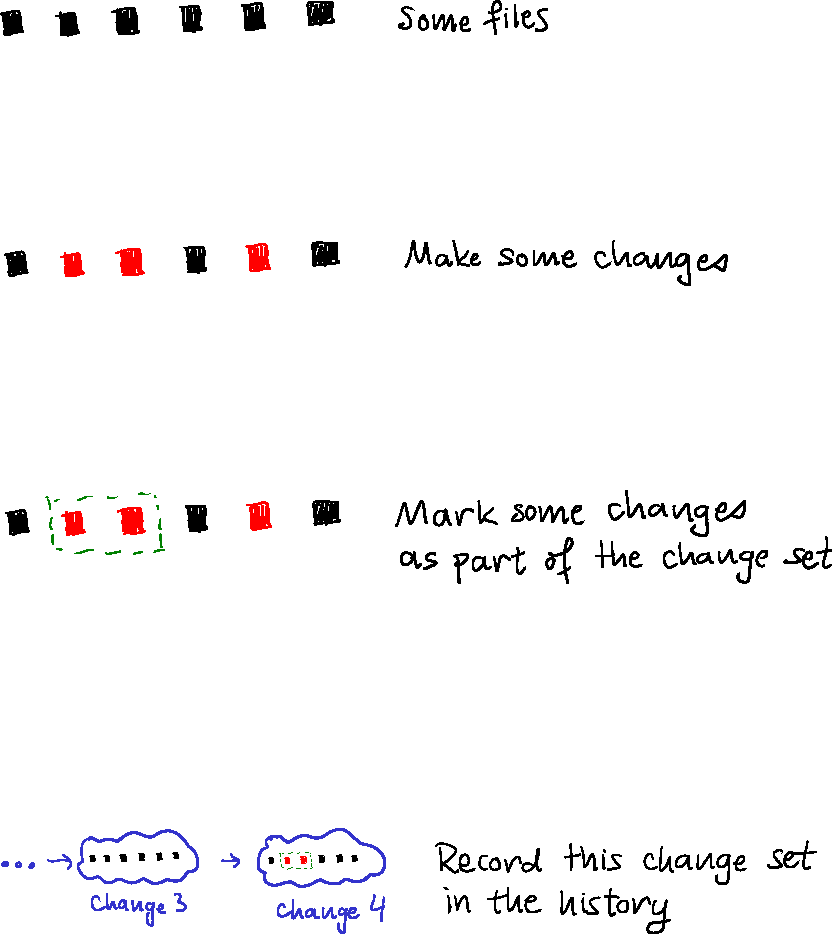
\includegraphics[width=270pt]{images/git_boxes.pdf} }}%
\only<2>{\centerline{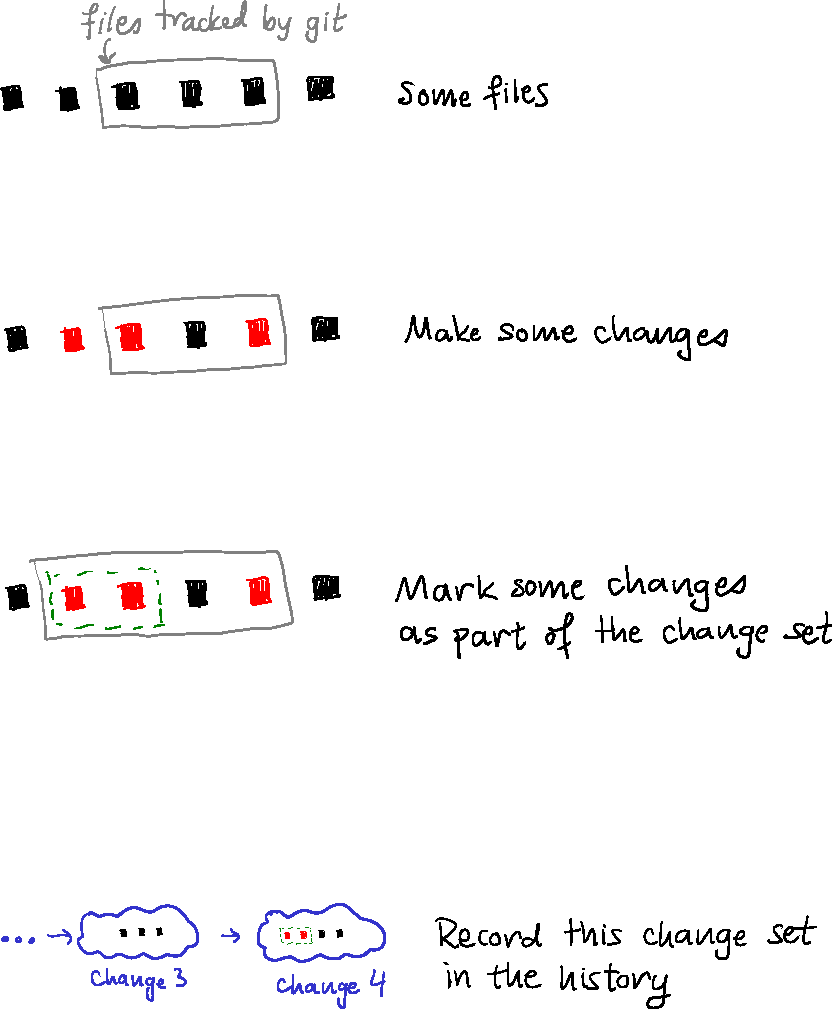
\includegraphics[width=270pt]{images/git_boxes2.pdf} }}%
\only<3>{\vspace{22pt}\centerline{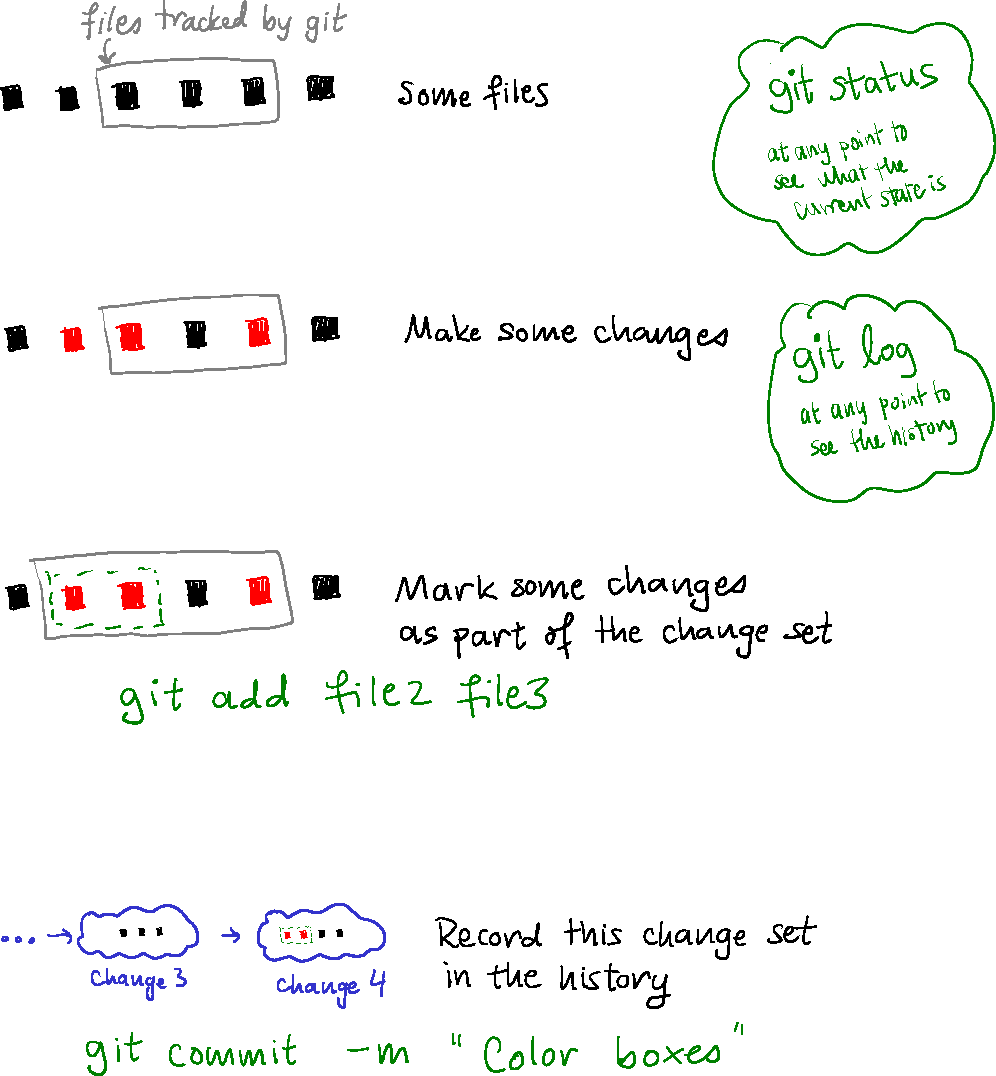
\includegraphics[width=300pt]{images/git_boxes4.pdf} }}%

\end{frame}

\begin{frame}[fragile] {Git: workflow with local and remote}
\only<1>{\centerline{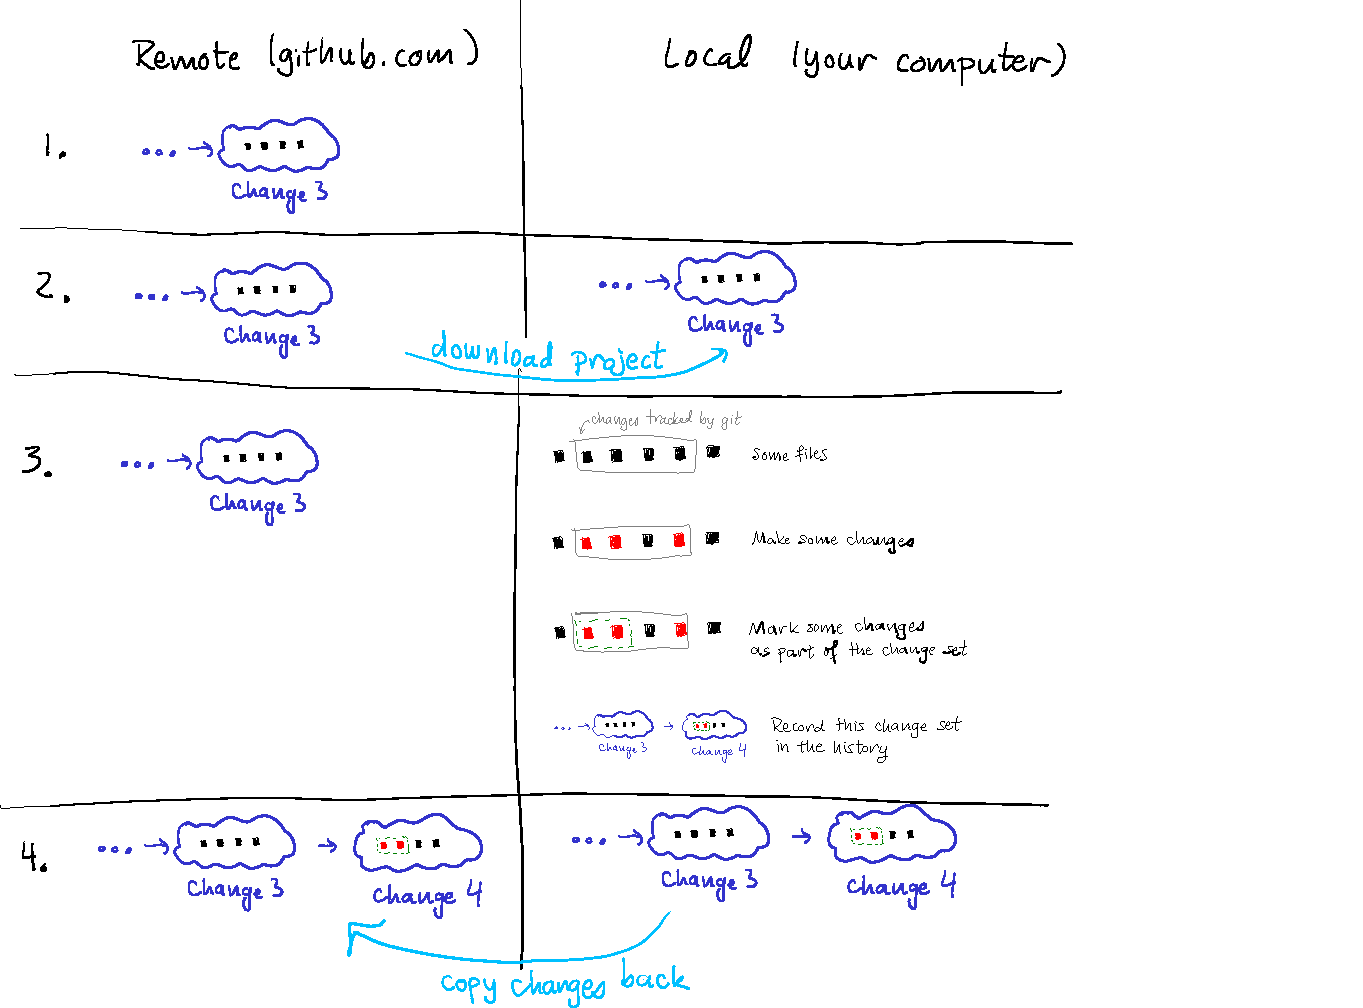
\includegraphics[width=330pt]{images/github2.pdf}}}
\only<2->{\centerline{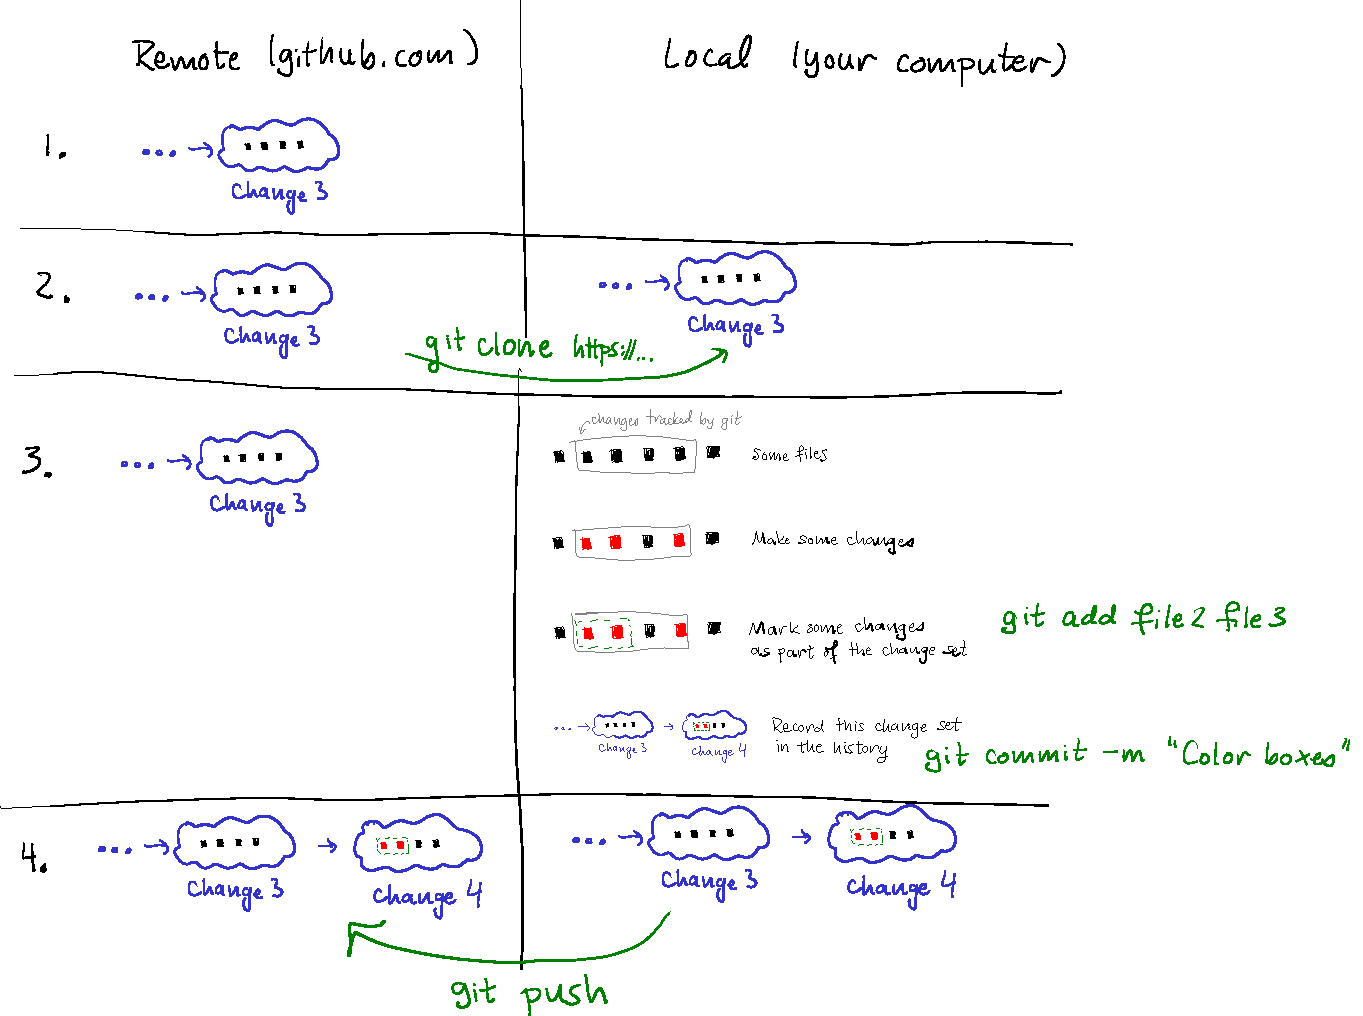
\includegraphics[width=330pt]{images/github3.pdf}}}
\only<3->{
\vspace{-5pt}

\begin{block}{Exercise 8}
\begin{enumerate} \scalefont{0.8}
\item \easycmd{git clone https://github.com/ebelmont/test}
\item Change to the {\tt test} directory
\uncover<4>{\item Make a new file in the {\tt test} directory with your name as the filename (e.g.
{\tt eva.txt}). Put some text in it and save.
\item \easycmd{git add} the file {\hspace{10pt}\color{mgray}if you didn't use tab completion, do
it again!}
\item Commit

\item Run \easycmd{git push} and enter your github username and token (if you
followed yesterday's email)
}
\end{enumerate}
\end{block}
\vspace{-20pt}
}
\end{frame}

\begin{frame} [fragile]{Missing from the picture: {\tt git pull}}
\centerline{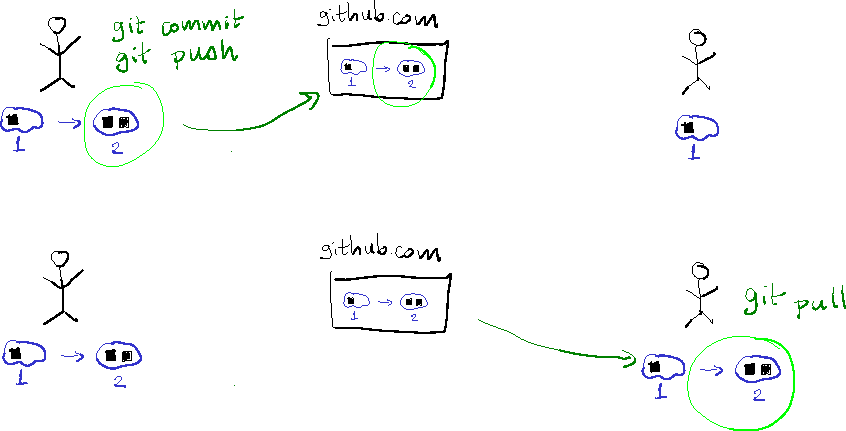
\includegraphics[width=330pt]{images/pull.pdf}}
\end{frame}

\begin{frame} [fragile] {Moral of the story: {\tt git pull} and then {\tt git push}}
\vspace{20pt}
\only<1>{\vspace{-140pt}\centerline{\hspace{-20pt}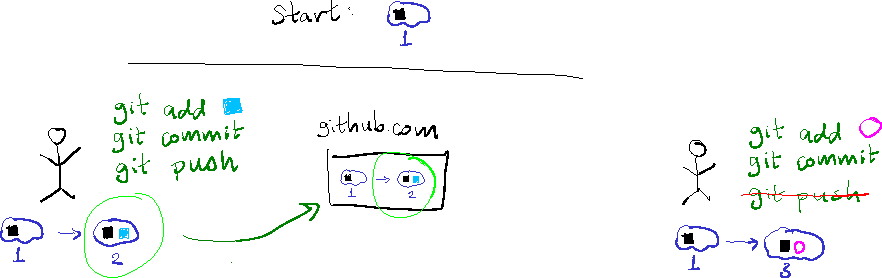
\includegraphics[width=310pt]{images/pull2.pdf}}}
\only<2->{\centerline{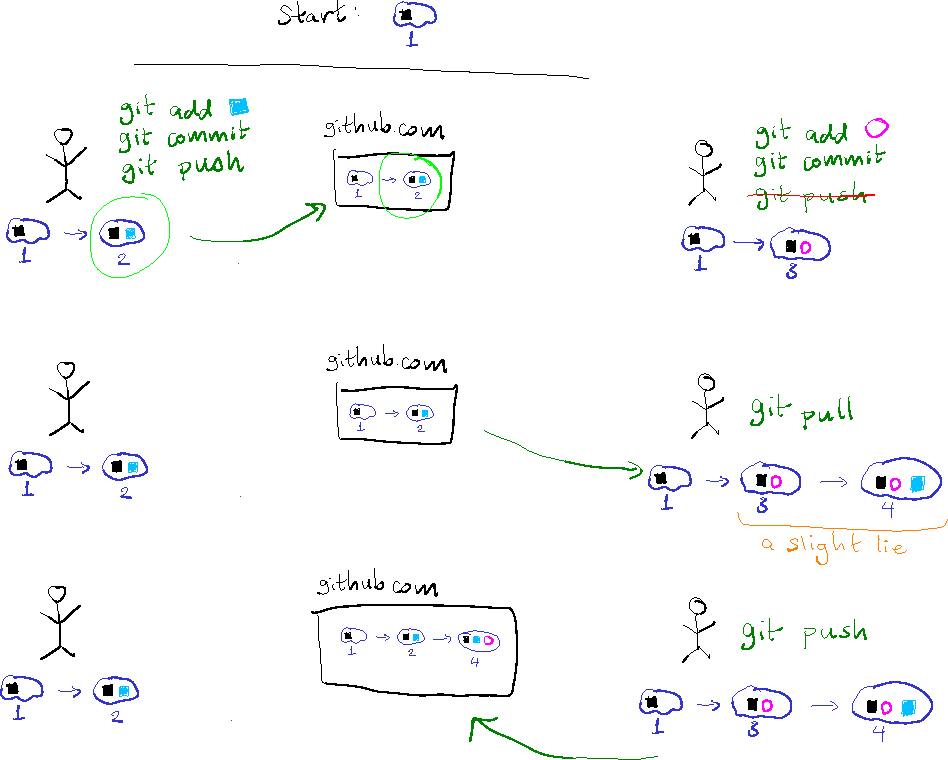
\includegraphics[width=330pt]{images/pull3.pdf}}}
\uncover<3>{
\vspace{-20pt}
{\bf Workflow recap:}
\vspace{-15pt}
\begin{enumerate} 
\item \easycmd{git clone url} (once)
\item Make edits
\item Add files and commit
\item \easycmd{git pull} \hspace{10pt} {\scalefont{0.8}\color{mgray}(let's all
choose \easycmd{git config pull.rebase false})}
\item \easycmd{git push}
\item Go to step 2 (and \easycmd{git pull} first if it's been a little while to make
sure you have up-to-date copy)
\end{enumerate}
}
\end{frame}

\begin{frame}[fragile] {Merging: what if two people change the same file?}
\begin{itemize} 
\item Often it ``just works''
\vspace{30pt}
\item Sometimes it causes a {\bf merge conflict}  that needs to be fixed
manually
\begin{itemize} 
\item Edit the offending file, removing the
\\\verb=<<<<<< HEAD= 
\\line etc., so that it's what you want
\item Add and commit the offending file
\item {\color{mgray}If you chose \cmd{git config pull.rebase true}, do
\\\cmd{git rebase --continue}
\\instead of committing}
\end{itemize}
\end{itemize}
\end{frame}

\begin{frame} {Another common issue: {\tt git pull} with conflicting uncommitted changes}
\centerline{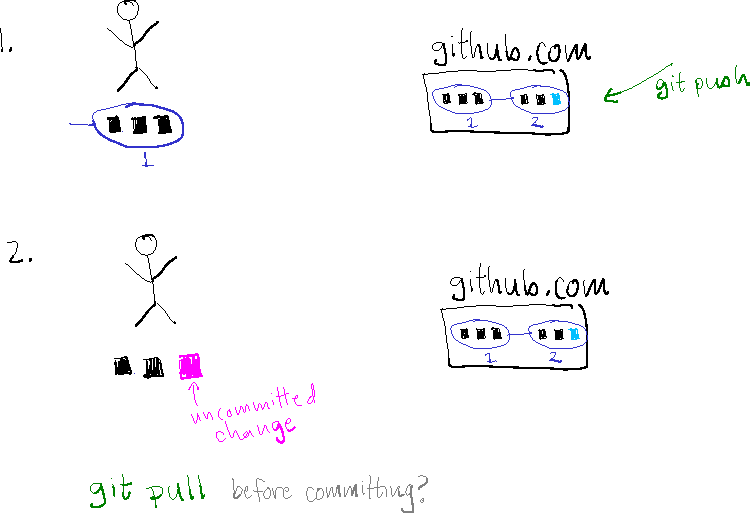
\includegraphics[width=200pt]{images/uncommitted_conflict.pdf} }

\pause
\vspace{40pt}

\centerline{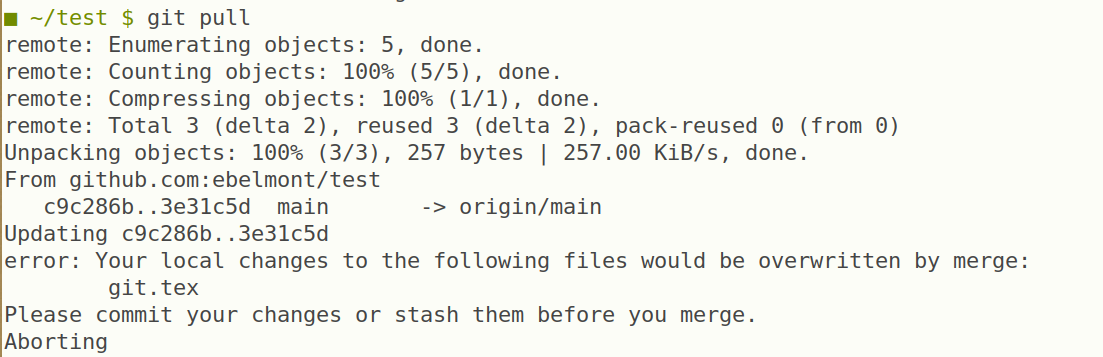
\includegraphics[width=250pt]{images/uncommitted_error.png} }
\end{frame}

\begin{frame}[fragile] {Branches}
\only<1>{\vspace{-290pt}\centerline{\hspace{-40pt}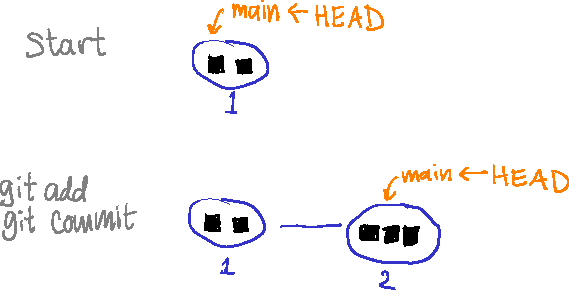
\includegraphics[width=160pt]{images/branches1.pdf}}}
\only<2>{\vspace{-190pt}\centerline{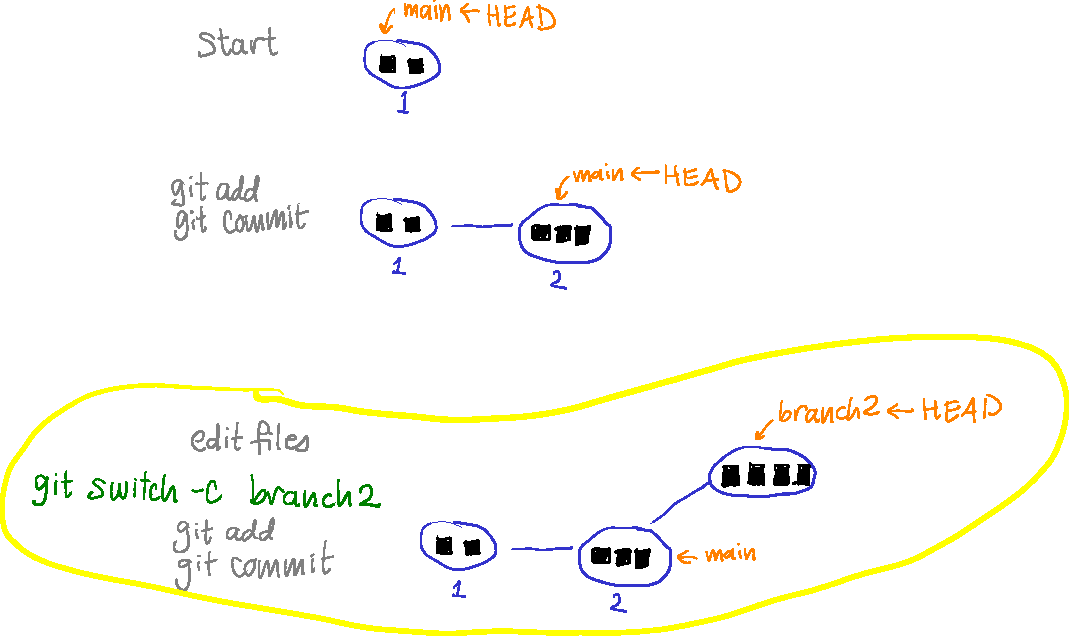
\includegraphics[width=300pt]{images/branches2.pdf}}}
\only<3>{\vspace{-100pt}\centerline{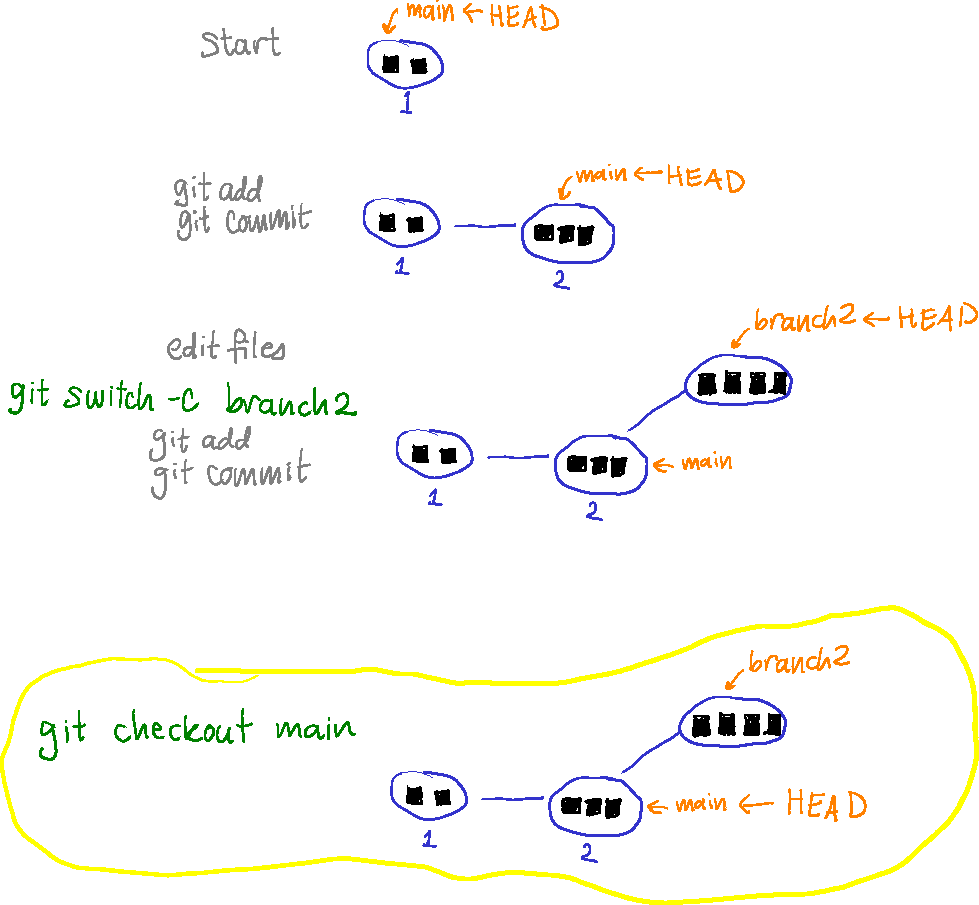
\includegraphics[width=290pt]{images/branches3.pdf}}}
\only<4->{\vspace{-50pt}\centerline{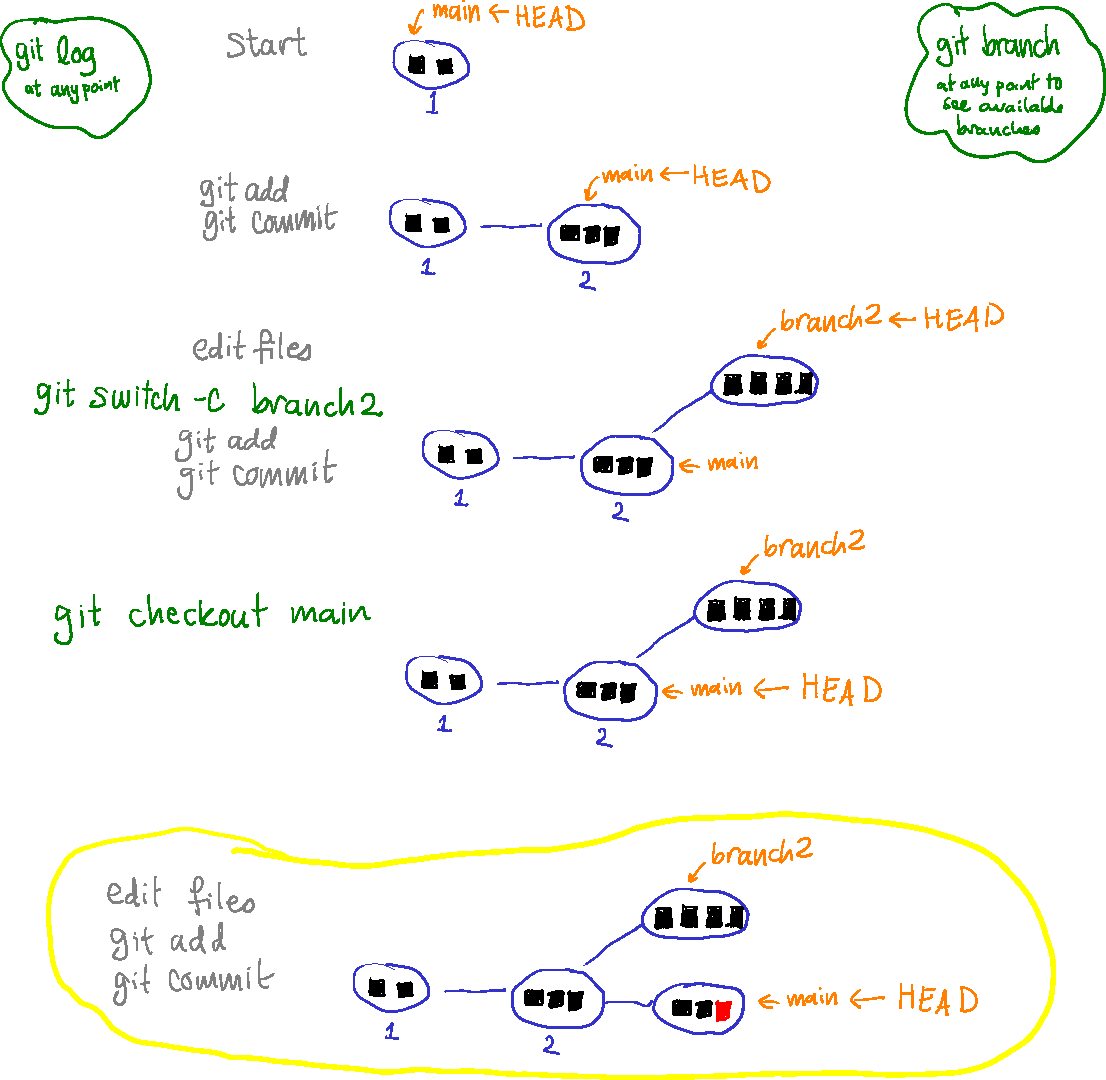
\includegraphics[width=310pt]{images/branches4.pdf}}}
\only<5>{
\begin{block}{Exercise 9}
What is the common ancestor of the two commits that were merged in
the last example?
\\\scalefont{0.8}Hint: use \easycmd{git log} to get the two parents of the merge
commit. The parent of commit {\tt 1234} is {\tt 1234}\string^, and you can use
\easycmd{git show 1234\string^} to expand the \string^.
\end{block}
\vspace{-70pt}
}
\end{frame}

\begin{frame} {{\tt git} in vscode}
\hspace{-20pt}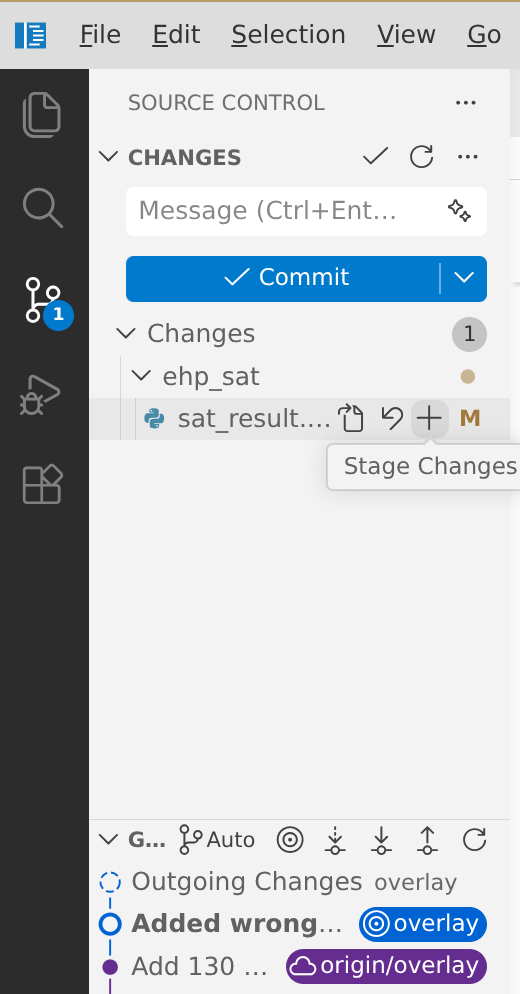
\includegraphics[width=120pt]{images/vscode1.png}
\hspace{50pt}
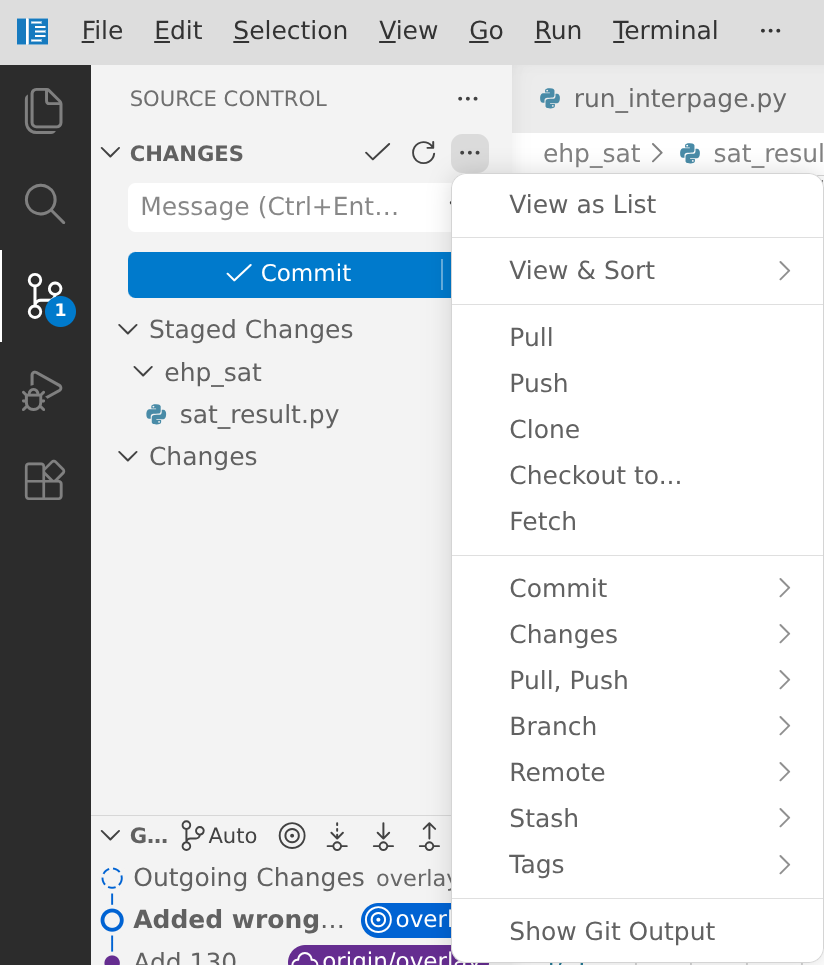
\includegraphics[width=160pt]{images/vscode2.png}\hspace{-80pt}


\vfill

\hspace{-20pt}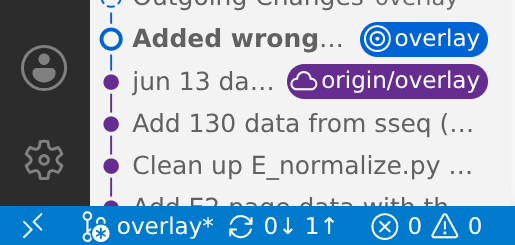
\includegraphics[width=120pt]{images/vscode3.png}
\vspace{-40pt}
\end{frame}

\begin{frame} {Takeaways}
\begin{block}{Standard workflow}
\easycmd{git pull}

Edit files

\easycmd{git add} changed files

\easycmd{git commit -m} ``Some useful message''

\easycmd{git pull}

\easycmd{git push}
\end{block}

\vspace{30pt}

\begin{block}{Confused?}
\easycmd{git status}
\end{block}
\end{frame}


\begin{frame}[fragile] {More useful things}
\begin{itemize} 
\item \cmd{git difftool} {\hspace{10pt}\color{mgray} Show un-staged (i.e., not {git add}ed) changes}
\vspace{18pt}
\item \cmd{git difftool --cached} {\hspace{10pt}\color{mgray} Show added but not
committed changes}
\vspace{18pt}
\item \cmd{git difftool HEAD HEAD^} {\hspace{10pt}\color{mgray} Show
changes between current version and previous commit}
\vspace{18pt}

\item {\tt .gitignore} (to make git \emph{not} track changes from certain files, e.g.
*.aux, *.log)

\url{https://docs.github.com/en/get-started/git-basics/ignoring-files}
\vspace{18pt}
\item Messed up with un-committed changes and want to go back to the last
commit?
\\\cmd{git reset --hard}
\\(but be {\bf REALLY} careful with this one, as it will permanently delete uncommitted changes)

\vspace{18pt}
\item {\tt {ssh}} keys for authentication (if you get tired of typing the
authentication token)

\url{https://docs.github.com/en/authentication/connecting-to-github-with-ssh/adding-a-new-ssh-key-to-your-github-account}

\end{itemize}
\end{frame}

\end{document}

